\tikzset{every picture/.style={line width=0.75pt}} %set default line width to 0.75pt        

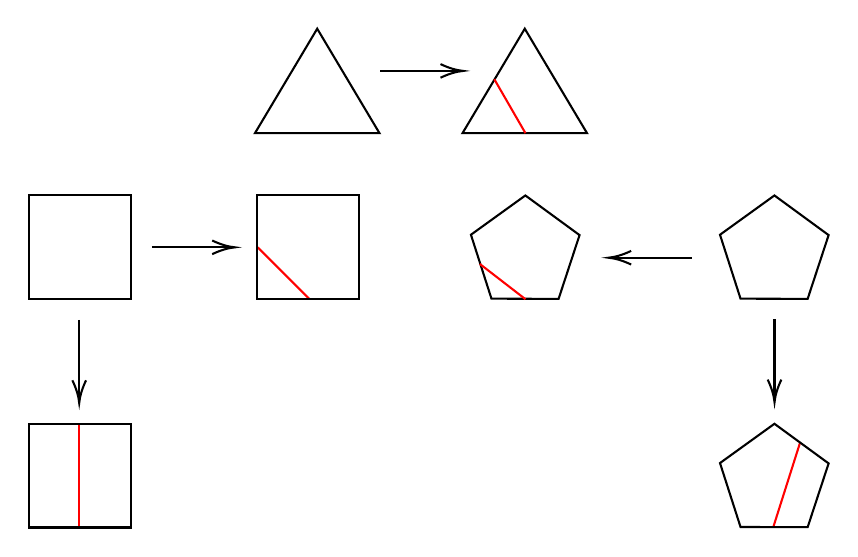
\begin{tikzpicture}[x=0.75pt,y=0.75pt,yscale=-1,xscale=1]
%uncomment if require: \path (0,300); %set diagram left start at 0, and has height of 300

%Shape: Triangle [id:dp053948984035182] 
\draw   (360,20) -- (390,70.33) -- (330,70.33) -- cycle ;
%Straight Lines [id:da38899678532814896] 
\draw [color={rgb, 255:red, 255; green, 0; blue, 0 }  ,draw opacity=1 ]   (345.33,44.33) -- (360.33,70.33) ;
%Shape: Triangle [id:dp9123444492379096] 
\draw   (260,20) -- (290,70.33) -- (230,70.33) -- cycle ;
%Straight Lines [id:da3333274202694039] 
\draw    (290.33,40.33) -- (328.33,40.33) ;
\draw [shift={(330.33,40.33)}, rotate = 180] [color={rgb, 255:red, 0; green, 0; blue, 0 }  ][line width=0.75]    (10.93,-3.29) .. controls (6.95,-1.4) and (3.31,-0.3) .. (0,0) .. controls (3.31,0.3) and (6.95,1.4) .. (10.93,3.29)   ;
%Shape: Rectangle [id:dp658152795456475] 
\draw   (121,100.33) -- (170.33,100.33) -- (170.33,150.33) -- (121,150.33) -- cycle ;
%Straight Lines [id:da4178479503741537] 
\draw [color={rgb, 255:red, 255; green, 0; blue, 0 }  ,draw opacity=1 ]   (231.33,125.33) -- (256.33,150.33) ;
%Shape: Rectangle [id:dp13970992998037612] 
\draw   (231,100.33) -- (280.33,100.33) -- (280.33,150.33) -- (231,150.33) -- cycle ;
%Straight Lines [id:da7168002284640573] 
\draw    (180.33,125.33) -- (218.33,125.33) ;
\draw [shift={(220.33,125.33)}, rotate = 180] [color={rgb, 255:red, 0; green, 0; blue, 0 }  ][line width=0.75]    (10.93,-3.29) .. controls (6.95,-1.4) and (3.31,-0.3) .. (0,0) .. controls (3.31,0.3) and (6.95,1.4) .. (10.93,3.29)   ;
%Straight Lines [id:da6092781758766023] 
\draw [color={rgb, 255:red, 255; green, 0; blue, 0 }  ,draw opacity=1 ]   (145.33,210.33) -- (145.33,260.33) ;
%Shape: Rectangle [id:dp4001001964953048] 
\draw   (121,210.33) -- (170.33,210.33) -- (170.33,260.33) -- (121,260.33) -- cycle ;
%Straight Lines [id:da7178391716405099] 
\draw    (145.33,160.33) -- (145.33,198.33) ;
\draw [shift={(145.33,200.33)}, rotate = 270] [color={rgb, 255:red, 0; green, 0; blue, 0 }  ][line width=0.75]    (10.93,-3.29) .. controls (6.95,-1.4) and (3.31,-0.3) .. (0,0) .. controls (3.31,0.3) and (6.95,1.4) .. (10.93,3.29)   ;
%Shape: Regular Polygon [id:dp33160480080690447] 
\draw   (360.29,100.34) -- (386.39,119.44) -- (376.29,150.16) -- (343.95,150.06) -- (334.06,119.26) -- cycle ;
%Straight Lines [id:da45618558829906886] 
\draw [color={rgb, 255:red, 255; green, 0; blue, 0 }  ,draw opacity=1 ]   (338.33,133.33) -- (360.33,150.33) ;
%Straight Lines [id:da6044104143635626] 
\draw [color={rgb, 255:red, 255; green, 0; blue, 0 }  ,draw opacity=1 ]   (492.67,219.33) -- (479.67,260.33) ;
%Straight Lines [id:da4256082202655984] 
\draw    (480.33,160) -- (480.33,198) ;
\draw [shift={(480.33,200)}, rotate = 270] [color={rgb, 255:red, 0; green, 0; blue, 0 }  ][line width=0.75]    (10.93,-3.29) .. controls (6.95,-1.4) and (3.31,-0.3) .. (0,0) .. controls (3.31,0.3) and (6.95,1.4) .. (10.93,3.29)   ;
%Straight Lines [id:da5844395653617523] 
\draw    (440.33,130.33) -- (402.33,130.33) ;
\draw [shift={(400.33,130.33)}, rotate = 360] [color={rgb, 255:red, 0; green, 0; blue, 0 }  ][line width=0.75]    (10.93,-3.29) .. controls (6.95,-1.4) and (3.31,-0.3) .. (0,0) .. controls (3.31,0.3) and (6.95,1.4) .. (10.93,3.29)   ;
%Shape: Regular Polygon [id:dp2820123358797324] 
\draw   (480.29,100.34) -- (506.39,119.44) -- (496.29,150.16) -- (463.95,150.06) -- (454.06,119.26) -- cycle ;
%Shape: Regular Polygon [id:dp4174131602657527] 
\draw   (480.29,210.34) -- (506.39,229.44) -- (496.29,260.16) -- (463.95,260.06) -- (454.06,229.26) -- cycle ;

\end{tikzpicture}
